\section{Results} \label{sec:results}

\subsection{CTF shows which sources potentially contribute to the extracted ROI time series}

In this section, we illustrate how CTF can be used to understand the pattern of RFS for any brain area of interest and a linear ROI extraction pipeline. First, we notice that every combination of linear methods for the extraction of ROI time series can be represented by an equivalent spatial filter (Fig. \ref{fig:general_idea}\tocheck{A}). For the commonly used two-step approach, the spatial filter is obtained as the product of the inverse operator matrix (e.g., eLORETA) and a vector of aggregation weights for sources within ROIs (e.g., a vector of ones for averaging). In Fig. \ref{fig:minimal-example}\tocheck{A}, one can clearly observe that the corresponding spatial filters differ between extraction pipelines. Still, it is unclear from the topomaps alone how these differences affect the extracted signal.

To improve the interpretability, we can multiply the spatial filter by a leadfield matrix and obtain the CTF. The CTF contains a value for each source in the forward model and describes the potential contribution of that source to the extracted ROI time series. In contrast to spatial filters, the CTFs shown in Fig. \ref{fig:minimal-example}\tocheck{B} provide more information and suggest that mean weights might even lead to cancellation of source activity originating from the opposite walls of the postcentral gyrus. In particular, if three sources (shown in \tocheck{green, black, and violet}) are placed, CTF values at the source locations show the expected amount of variance that each of the sources will explain in the extracted ROI time series (Fig. \ref{fig:minimal-example}\tocheck{C}, theory). The predictions imply that the main contributors to the extracted signal will differ between approaches, potentially leading to differences in subsequent analyses for this configuration of sources.

However, CTF reflects only the potential impact of the source, and the amplitude of the source activity also matters in practice. If we run a simulation with equal variance of source activity for all three sources, the extraction quality obtained in the simulations will match the CTF-based predictions very closely (theory and simulation match in Fig. \ref{fig:minimal-example}\tocheck{C}). However, if we introduce unequal variance between the sources, for example, by increasing the amplitude of the \tocheck{green} source by \tocheck{\simExpAUnequalStd}~times, its contribution to the extracted time series will exceed theoretical expectations (theory in Fig. \ref{fig:minimal-example}\tocheck{C} does not match simulations in Fig. \ref{fig:minimal-example}\tocheck{D}). By incorporating prior knowledge in the form of the source covariance matrix, it is possible to improve the CTF-based evaluation (theory and simulation match again in Fig. \ref{fig:minimal-example}\tocheck{D}).

\begin{figure}[htbp]
    \centering
    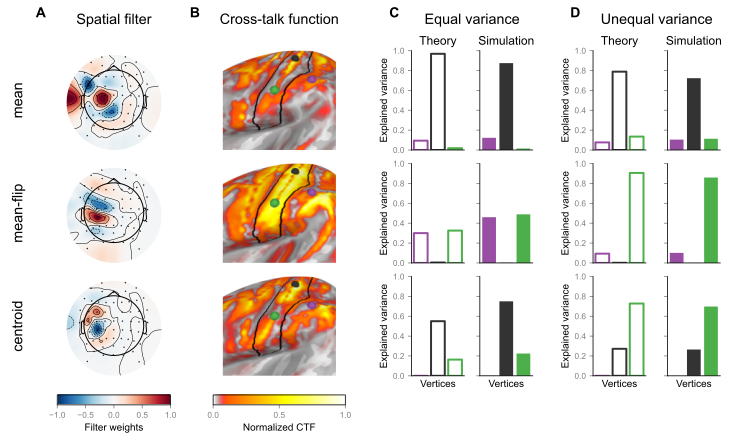
\includegraphics[width=\linewidth]{figures/fig3_minimal_example.png}
    \caption{CTF can be used to investigate differences between pipelines for the extraction of ROI activity, as it shows which sources can potentially contribute to the extracted signal. Rows correspond to different aggregation methods (mean, mean-flip, centroid) after inverse modeling with eLORETA. (A) An equivalent spatial filter can represent linear pipelines for the extraction of ROI activity. (B) CTFs for each pipeline (squared element-wise). Dots show the location of sources in simulations for Panels C and D. (C) Under the assumption of equal variance, squared CTF values at the location of each simulated source correspond to the amount of variance of the ROI time series that source explains. (D) To account for unequal source variances, a source covariance matrix must be used when calculating the CTF.}
    \label{fig:minimal-example}
\end{figure}

\subsection{CTF ratio as a metric of extraction quality: theory}

In the previous section, we showed how CTF values at the exact location of the simulated sources explain which sources may contribute to the extracted ROI time series. Since the ground-truth source locations are usually unknown in resting-state data, it is more practically relevant to consider the entire region rather than focus on specific locations.

For the interpretation of the results, the main contributors to the extracted time series must be located in the considered ROI and not in other areas of the brain. Using CTF, we can assess the fidelity of extracted time series for any spatial filter by estimating how much of the total power of the extracted signal potentially originates from the ROI. We refer to this metric as the CTF ratio (Eq. \ref{eq:ctf-ratio}), and examples of CTFs with low and high ratios are shown in Fig. \ref{fig:general_idea}\tocheck{D}. By default, the CTF ratio is calculated assuming unit activity strength for all sources. However, any prior knowledge about the source activity can also be incorporated in the calculations.

Through optimization, it is possible to obtain a theoretical upper limit of the CTF ratio for a given lead field and ROI. Importantly, this limit cannot be exceeded by any linear spatial filter. In Fig. \ref{fig:ctf-metrics}\tocheck{A}, we show the upper limits of the CTF ratio for the DK and Schaefer parcellations. The maximal CTF ratio is much smaller in deeper regions farther from the scalp surface and thus from the recording sensors (the medial wall of both hemispheres and the insula). In addition, ROIs from the Schaefer parcellation generally exhibit a lower CTF ratio than those from the DK parcellation, in part due to differences in ROI size. These factors are illustrated for the DK parcellation in Fig. \ref{fig:ctf-metrics}\tocheck{D} and Fig. \ref{fig:ctf-metrics}\tocheck{E}, respectively. Finally, we show that the upper limit of the CTF ratio increases with the number of EEG sensors, but the increase is less pronounced for ROIs with a low CTF ratio (Fig. \ref{fig:ctf-metrics}\tocheck{F}).

As shown in Fig. \ref{fig:ctf-metrics}\tocheck{B}, the theoretical limits of the CTF ratio are not reached by commonly used approaches, which is at least partially caused by the applied regularization. However, the spatial distribution of the CTF ratio remains non-uniform, with deeper regions showing a lower CTF ratio. If we were to select methods that yield the highest CTF ratio across different ROIs of the DK parcellation, we would find that different methods benefit different ROIs (Fig. \ref{fig:ctf-metrics}\tocheck{C}). Therefore, the question about an optimal extraction pipeline is likely to have an ROI-specific rather than a one-size-fits-all answer.

\begin{figure}[htbp]
    \centering
    \includegraphics[width=\linewidth]{figures/fig4_ctf_metrics.png}
    \caption{The theoretical upper limit and achieved values of the CTF ratio for the considered data-independent pipelines. (A) The upper limit of the CTF ratio for Desikan-Killiany (DK) and Schaefer parcellations. (B) Achieved values of the CTF ratio for the considered pipelines and DK parcellation. (C) The pipeline that showed the highest CTF ratio for each ROI of the DK parcellation. (D) The upper limit of the CTF ratio decreases as the average distance from sources within the ROI to the recording sensors increases. (E) The upper limit of the CTF ratio is higher for larger ROIs. (F) The upper limit of the CTF ratio increases with the number of EEG sensors. In Panels D-F, ROIs from the DK parcellation were considered.}
    \label{fig:ctf-metrics}
\end{figure}

\subsection{CTF ratio as a metric of extraction quality: validation in simulations}

We validated the idea behind the CTF ratio in simulations with distributed ground-truth source activity and used simulation parameters derived from real data, where possible. In particular, we tested whether the CTF ratio can explain differences in extraction quality between regions of interest and between approaches for the extraction of ROI time series. In addition, we empirically evaluated the reliability of CTF-based explanations when the assumption of equal activity strength for all sources does not hold.

To systemically assess the extraction quality, we simulated one ground-truth source of alpha (\tocheck{\fminAlphaHz--\fmaxAlphaHz}~Hz) activity at a randomly selected location in each ROI of the DK parcellation, added \tocheck{\simNumNoiseSources}~point-like sources of 1/f activity at random locations in the cortex, and projected the resulting source activity to the sensor space. After that, we applied several commonly used approaches for the extraction of ROI time series and, for each ROI, evaluated the correlation between the extracted signal and the ground-truth activity of the alpha source within the ROI.

By default, the CTF calculation assumes unit activity strength and zero covariance between all sources in the cortex. However, this assumption is likely violated in real M/EEG data, since, for example, sources in occipital areas typically exhibit higher alpha power in resting-state data, and connectivity can be observed even between distant regions. To test the potential value of CTF ratio in the case of violated underlying assumptions, we performed several experiments (Fig. \ref{fig:simulation-workflow}\tocheck{B}), in which we incrementally violated of the unit-activity-strength assumption by introducing a non-uniform distribution of source variance across regions, manipulating the size of alpha sources, introducing ground-truth connectivity between sources in different ROIs, and manipulating the signal-to-noise ratio in source and sensor space.

To verify that the CTF ratio predicts the differences in extraction quality between regions, we evaluated the correlation between theoretical (CTF-based) and simulation-based estimates of extraction quality across all areas of the parcellation. The results of this analysis are shown in Fig. \ref{fig:experiments}\tocheck{A}. As expected (see Fig.~\ref{fig:minimal-example}), when the CTF ratio is evaluated exactly at the ground truth location of each source with full knowledge of the source covariance matrix, the correlation with the results of simulations is almost perfect (dashed grey lines). As soon as we switch to using ROIs instead of sources, the correlation decreases slightly but remains high (solid grey lines). In addition, this correlation begins to depend on experimental conditions and worsens as the introduced deviations become stronger. A notable exception to these results is the effect of source size: as source size increases, the area of the source approaches the area of the corresponding ROI, making ROI-based and source-based evaluations more similar. Finally, when the CTF ratio is evaluated without information about the source covariance matrix and on a different source grid (solid black lines), the correlation drops to around 0.6 but remains relatively stable across all experiments.

For the latter case, we also studied the differences between extraction pipelines (Fig. \ref{fig:experiments}\tocheck{B}). Generally, the correlation values were similar for LCMV and eLORETA. Among ROI aggregation weights, CTF-based predictions showed the lowest correlation with simulation-based estimates for averaging (mean). In addition, this method also shows different behavior in Experiment 2, in which the source size was varied. Altogether, these results might suggest a misestimation of the cancellation of activity from sources with opposite orientations when averaging is used.

\begin{figure}[htbp]
    \centering
    \includegraphics[width=\linewidth]{figures/fig5_experiments.png}
    \caption{CTF ratio predicts the extraction quality (measured as the Pearson correlation between extracted ROI time series and simulated ground-truth activity) in simulations, even when the default assumption of uncorrelated unit-variance sources is violated (Experiments 1-4b). (A) Correlation between the CTF ratio and extraction quality across ROIs of the DK parcellation. The results were averaged over eight pipelines for the extraction of ROI activity. (B) Correlation between the CTF ratio and extraction quality, shown separately for each pipeline, in the case when a different source grid (compared to one used for simulating the data) and no knowledge about the source covariance matrix were used for computing the CTF (black line in Panel A). Abbreviations: EO --- eyes-open condition, EC --- eyes-closed condition, SNR --- signal-to-noise ratio.}
    \label{fig:experiments}
\end{figure}

\subsection{CTF explains patterns of spurious coherence (SC) better than the distance between ROIs}

From this point, we switch our focus to the estimation of inter-regional connectivity and the information that CTF can provide. One direct consequence of the remaining field spread (RFS) in the context of connectivity is the detection of spurious connectivity (e.g., as measured by coherence). When the spatial filters for two ROIs capture the same sources, high coherence may be observed even in the absence of a genuine underlying interaction. Since field spread affects commonly investigated frequencies similarly, this effect manifests as a vertical shift of the coherence spectra as the distance between the regions decreases (Fig. \ref{fig:spurious-coherence}\tocheck{A}). As CTF shows the amount of RFS, it can be used to estimate the degree of spurious coherence that would occur if no genuine ground-truth connections were present on the source level.

We compared the CTF-based estimates of SC (Eq. \ref{eq:spurious-coherence}) with the values of SC estimated from the resting-state EEG data of the LEMON dataset using permutations. To quantify the amount of SC for each connectivity edge, we generated surrogate data using the permutation approach introduced by \cite{Shahbazi2010}. This approach destroys all genuine interactions, leaving only the SC caused by the field spread. The estimates of SC for three data-independent pipelines are shown in Fig. \ref{fig:spurious-coherence}\tocheck{E}. Fig. \ref{fig:spurious-coherence}\tocheck{D} shows the CTF-based estimates of SC for the same pipelines. Additionally, we considered a competing model based on the distance between the centers of gravity of ROIs, since one might intuitively expect that SC is high between neighboring regions and decreases with distance (Fig. \ref{fig:spurious-coherence}\tocheck{C}).

We evaluated the correlation between model-based estimates of SC (based either on CTF or on the distance between ROI centroids) and estimates obtained from the surrogate data. As shown in Fig. \ref{fig:spurious-coherence}\tocheck{B}, CTF-based estimates showed a higher correlation with surrogate data than distance-based estimates (on average across considered pipelines). While the distance-based model cannot explain the difference between extraction methods by construction (distance does not depend on the extraction method), CTF also explained on average about \scCTFDeltaEV\% of the variance in pipeline-specific differences in SC (Fig. \ref{fig:spurious-coherence}\tocheck{B}, delta). The correlation values were similar in the eyes-closed and eyes-open conditions. The detailed results are presented in Table \ref{supp-tab:spurious-coherence}.

\begin{figure}[htbp]
    \centering
    \includegraphics[width=\linewidth]{figures/fig6_spurious_coherence.png}
    \caption{CTF predicts the degree of spurious coherence (SC) between extracted ROI time series better than the distance between ROI centroids. (A) In real data, SC manifests as a vertical shift of the grand-average coherence spectra, as shown here using resting-state data of \tocheck{\lemonNumIncluded} LEMON participants (eyes closed condition) for the combination of eLORETA and mean-flip. The values of SC are averaged over connectivity edges within distance-based bins (shown in the inset plot). (B) CTF explains more variance in the values of SC derived from surrogate data than the distance between ROI centers. In addition, CTF explains a considerable amount of difference in SC between the extraction pipelines. In both plots, the correlation values are averaged over three data-independent pipelines. (C) Distance-based estimates of SC for all pairs of ROIs from the DK parcellation. (D) CTF-based estimates of SC for the DK parcellation and three data-independent pipelines for the extraction of ROI activity. (E) Estimates of SC derived from surrogate data for the same parcellation and methods. In Panels C-E, ROIs are sorted alphabetically. Abbreviations: EO --- eyes-open condition, EC --- eyes-closed condition.}
    \label{fig:spurious-coherence}
\end{figure}

\subsection{Recovery of ground-truth connectivity is not uniform across the cortex}

In addition to spurious coherence, the CTF also provides information about the potential contribution of each pair of sources to the estimated inter-regional connectivity. Since extracted time series for ROIs with low CTF ratios are likely to contain activity from other ROIs, they are also more likely to capture ground-truth interactions between other brain regions. To illustrate this, we performed a simulation with a ground-truth connection between two deep ROIs with a low CTF ratio (denoted as target in Fig. \ref{fig:example-connectivity}). As shown in Fig. \ref{fig:example-connectivity}\tocheck{A} for an exemplary extraction pipeline (eLORETA, mean-flip), the CTF for the target ROIs spreads well beyond these to other brain areas. Based on Fig. \ref{fig:example-connectivity}\tocheck{A}, we picked two more ROIs and added another ground-truth connection between them (denoted as interference). The effect of RFS is asymmetric: the CTFs of the interfering ROIs are concentrated within these ROIs and are not (to a large extent) expected to pick up the activity of the target ones (Fig. \ref{fig:example-connectivity}\tocheck{C}).

To investigate the effect of such asymmetry on the estimated connectivity values, we varied the presence of ground-truth interactions between the target and interfering ROIs by simulating configurations with no connections, one connection (either the target or the interfering one), or both. In Fig. \ref{fig:example-connectivity}\tocheck{B} and Fig. \ref{fig:example-connectivity}\tocheck{D}, we show the spectra of the estimated absolute ImCoh between the extracted time series of target and interfering ROIs, respectively. Notably, for both connections, ImCoh is high if and only if the interfering connection is present. As a result, both connections are dominated by ground-truth interference ImCoh, while the actual target ImCoh has a relatively small influence. This effect can be shown more generally with CTF by considering the contribution of each ground-truth ImCoh towards the estimated ImCoh between any pair of ROIs (Eq. \ref{eq:imcoh-mixing}). The main result remains the same: connections between ROIs with low CTF ratio are more likely to pick up interactions from the outside (Fig. \ref{supp-fig:imcoh-recovery}).

\begin{figure}[htbp]
    \centering
    \includegraphics[width=\linewidth]{figures/fig7_connectivity_example.png}
    \caption{The effect of remaining field spread (RFS) on ImCoh between ROIs can be asymmetric. One target and one interference connectivity edge were simulated using ROIs from the DK parcellation. (A) Target ROIs (highlighted in red) are displayed on top of the CTF (grey), which the combination of eLORETA and mean-flip has for these ROIs. Notice that the CTF values are high within the interference ROIs (highlighted in blue in Panel C). (B) As a result, the estimated ImCoh for the target connectivity edge strongly reacts to changes in the ground-truth connectivity of the interference edge. (C) The CTF of the interference ROIs is highly localized. (D) The interference edge mostly picks up its own connectivity in simulations.}
    \label{fig:example-connectivity}
\end{figure}

\subsection{CTF explains the connectivity patterns observed during RIFT}

Finally, we tested the predictions of CTF in real data from a steady-state visual stimulation paradigm. Flickering stimuli elicit a steady-state visual evoked response (SSVER) that exhibits a strong oscillatory-like component at the stimulation frequency. Previous research \citep{DiRusso2007, Spaak2024_paper} has shown that the main generators of SSVER are located in the primary visual cortex (V1), and their activity is strongly synchronized with the presented stimulus at the stimulation frequency (Fig. \ref{fig:rift-onestim}\tocheck{A}). This phenomenon allows one to embed ground-truth connectivity in real data by controlling the amplitude and phase of luminance modulation for the presented stimuli. In sensor space, the pattern of brain-stimulus coherence in the single-stimulus condition peaks in occipital areas, as shown in Fig. \ref{fig:rift-onestim}\tocheck{B}.

Due to RFS, we might observe coherence with the stimulus in other ROIs apart from V1, even if only V1 contains the main generators of SSVER. If this is the case, we should be able to predict the amount of coherence with CTF. To test this hypothesis, we used CTF to predict the expected coherence between each ROI and the external stimulus (assuming two point-like SSVER generators placed in V1) and compared the predictions with the results obtained from real data. For comparison, we considered a model with no RFS and another one in which RFS depends only on the distance between ROIs.

We evaluated the model fit only for connections that exceeded the noise floor (shown in Fig. \ref{supp-fig:noise-floor-onestim} and \ref{supp-fig:noise-floor-twostim} for brain-stimulus coherence and brain-brain ImCoh, respectively). The results of model comparison for brain-stimulus coherence are shown in Fig. \ref{fig:rift-onestim}\tocheck{D}. Both CTF-based and distance-based models predict brain-stimulus coherence values better than the model without RFS. However, only the CTF-based model additionally explained \riftOnestimDeltaEVMin--\riftOnestimDeltaEVMax\% of variance between extraction pipelines in estimated brain-stimulus coherence (see Tab. \ref{supp-tab:rift-onestim} for detailed results for all conditions). Predictions of the CTF-based model in comparison with real data estimates are shown in Fig. \ref{fig:rift-onestim}\tocheck{E}. Fig. \ref{fig:rift-onestim}\tocheck{C} shows the leadfield of SSVER generators, which resulted in the best model fit. The leadfield closely matches the sensor-space topomap of brain-stimulus coherence (Fig. \ref{fig:rift-onestim}\tocheck{B}). Similar results with slightly lower correlations were obtained for the brain-brain ImCoh in the two-stimuli condition (Fig. \ref{supp-fig:rift-twostim}, Tab. \ref{supp-tab:rift-twostim}).

\begin{figure}[htbp]
    \centering
    \includegraphics[width=\linewidth]{figures/fig8_rift_onestim.png}
    \caption{Whole-brain patterns of coherence between extracted ROI time series and the luminance of the flickering stimulus (brain-stimulus coherence) can be explained by two point-like sources located in V1 of both hemispheres using CTF. (A) When participants passively observe a flickering stimulus, a steady-state visual evoked response (SSVER) can be recorded. SSVER has a strong oscillatory-like component at the stimulation frequency (see time courses). This component is synchronized to the luminance modulation of the presented stimulus and can serve as a ground truth for connectivity benchmarks. (B) Sensor-space topomap of brain-stimulus coherence. (C) The lead field of the dipole configuration that led to the best fit for the CTF-based model. Notice its high similarity to the sensor-space pattern shown in Panel B. (D) CTF- and distance-based approaches explain a comparable amount of variance in raw values of brain-stimulus coherence. Still, CTF additionally explains the difference between pipelines for ROI extraction (delta). The correlation values were computed across pooled data from three data-independent extraction pipelines. (E) Theoretical predictions based on CTF and estimates of brain-stimulus coherence from real data are strongly positively correlated for all considered pipelines. $r_{fit}$ and $r_{all}$ denote the correlation values calculated for ROIs that exceeded the noise floor (red dots) and all ROIs (gray dots), respectively. For all panels, we used the data from the experimental condition with full luminance modulation (tagging type 1) and fixed starting phase.}
    \label{fig:rift-onestim}
\end{figure}
